%% bare_conf.tex
%% V1.4b
%% 2015/08/26
%% by Michael Shell
%% See:
%% http://www.michaelshell.org/
%% for current contact information.
%%
%% This is a skeleton file demonstrating the use of IEEEtran.cls
%% (requires IEEEtran.cls version 1.8b or later) with an IEEE
%% conference paper.
%%
%% Support sites:
%% http://www.michaelshell.org/tex/ieeetran/
%% http://www.ctan.org/pkg/ieeetran
%% and
%% http://www.ieee.org/

%%*************************************************************************
%% Legal Notice:
%% This code is offered as-is without any warranty either expressed or
%% implied; without even the implied warranty of MERCHANTABILITY or
%% FITNESS FOR A PARTICULAR PURPOSE! 
%% User assumes all risk.
%% In no event shall the IEEE or any contributor to this code be liable for
%% any damages or losses, including, but not limited to, incidental,
%% consequential, or any other damages, resulting from the use or misuse
%% of any information contained here.
%%
%% All comments are the opinions of their respective authors and are not
%% necessarily endorsed by the IEEE.
%%
%% This work is distributed under the LaTeX Project Public License (LPPL)
%% ( http://www.latex-project.org/ ) version 1.3, and may be freely used,
%% distributed and modified. A copy of the LPPL, version 1.3, is included
%% in the base LaTeX documentation of all distributions of LaTeX released
%% 2003/12/01 or later.
%% Retain all contribution notices and credits.
%% ** Modified files should be clearly indicated as such, including  **
%% ** renaming them and changing author support contact information. **
%%*************************************************************************

% *** Authors should verify (and, if needed, correct) their LaTeX system  ***
% *** with the testflow diagnostic prior to trusting their LaTeX platform ***
% *** with production work. The IEEE's font choices and paper sizes can   ***
% *** trigger bugs that do not appear when using other class files.       ***
% The testflow support page is at:
% http://www.michaelshell.org/tex/testflow/

\documentclass[conference]{IEEEtran}

% Make latex understand and use the typographic
% rules of the language used in the document.
\usepackage[english]{babel}
\usepackage[utf8]{inputenc}
% Choose the font encoding
\usepackage[T1]{fontenc}

% Use colour in tables
\usepackage[table]{xcolor}
\usepackage{array}
\usepackage{multirow}

% load a colour package
\usepackage{xcolor}
\definecolor{aaublue}{RGB}{33,26,82}% dark blue

% The standard graphics inclusion package
\definecolor{white}{RGB}{255,255,255} % define color white
\usepackage{graphicx}

% Set up how figure and table captions are displayed
\usepackage{caption}
\captionsetup{
  font=footnotesize,% set font size to footnotesize
  labelfont=bf % bold label (e.g., Figure 3.2) font
}

% Enable row combination in tables
\usepackage{multirow}

% Make space between table lines and text
\renewcommand{\arraystretch}{1.5}

% Make the standard latex tables look so much better
\usepackage{array,booktabs}



%%%%%%%%%%%%%%%%%%%%%%%%%%%%%%%%%%%%%%%%%%%%%%%%
% Mathematics
%%%%%%%%%%%%%%%%%%%%%%%%%%%%%%%%%%%%%%%%%%%%%%%%
% Defines new environments such as equation,
% align and split 
\usepackage{amsmath}
\usepackage{relsize}
% Adds new math symbols
\usepackage{amssymb}
% Use theorems in your document
% The ntheorem package is also used for the example environment
% When using thmmarks, amsmath must be an option as well. Otherwise \eqref doesn't work anymore.
\usepackage[framed,amsmath,thmmarks]{ntheorem}
\usepackage{cancel}

%%%%%%%%%%%%%%%%%%%%%%%%%%%%%%%%%%%%%%%%%%%%%%%%
% Page Layout
%%%%%%%%%%%%%%%%%%%%%%%%%%%%%%%%%%%%%%%%%%%%%%%%


%%%%%%%%%%%%%%%%%%%%%%%%%%%%%%%%%%%%%%%%%%%%%%%%
% Bibliography
%%%%%%%%%%%%%%%%%%%%%%%%%%%%%%%%%%%%%%%%%%%%%%%%
%%setting references (using numbers) and supporting i.a. Chicargo-style:
\usepackage{etex}
\usepackage{etoolbox}
\usepackage{keyval}
\usepackage{ifthen}
\usepackage{url}
\usepackage{csquotes}
\usepackage[backend=biber, url=true, doi=true, citestyle=ieee, bibstyle=ieee, sorting=none]{biblatex}
\addbibresource{setup/bibliography.bib}

%%%%%%%%%%%%%%%%%%%%%%%%%%%%%%%%%%%%%%%%%%%%%%%%
% Misc
%%%%%%%%%%%%%%%%%%%%%%%%%%%%%%%%%%%%%%%%%%%%%%%%

%%% Enables the use FiXme refferences. Syntax: \fxnote{...} %%%
\usepackage[footnote, draft, english, silent, nomargin]{fixme}
%With "final" instead of "draft" an error will ocure for every FiXme under compilation.

%%% allows use of lorem ipsum (generate i.e. pagagraph 1 to 5 with \lipsum[1-5]) %%%
\usepackage{lipsum}

%%% Enables figures with text wrapped tightly around it %%%
\usepackage{wrapfig}

\usepackage{float}
\usepackage{caption}
\usepackage{subcaption}
\usepackage{siunitx}
\sisetup{decimalsymbol=comma}
\sisetup{detect-weight}

\usepackage{enumitem}
%\usepackage[citestyle=authoryear,natbib=true]{biblatex}

% Figures - TIKZ
\usepackage{tikz}
\usetikzlibrary{shapes,arrows}
\usepackage[americanresistors,americaninductors,americancurrents, americanvoltages]{circuitikz}

% Wall of text logo
\newcommand{\walloftextalert}[0]{\includegraphics[width=\textwidth]{walloftext.png}}

\usepackage{pdfpages}
\usepackage{lastpage}
\usepackage{epstopdf}

\setlength{\headheight}{21pt}

\hfuzz=\maxdimen
\tolerance = 10000
\hbadness  = 10000

\usepackage{siunitx}
\graphicspath{{./figures/}}

%%%%%%%%%%%%%%%%%%%%%%%%%%%%%%%%%%%%%%%%%%%%%%%%%%%%%
%             UNITS, EQUATIONS AND TEXT             %
%%%%%%%%%%%%%%%%%%%%%%%%%%%%%%%%%%%%%%%%%%%%%%%%%%%%%
%Units:
\newcommand{\unit}[1]{&& \left[\si{#1}\right]} %\newcommand{\unit}[1]{[\si{#1}]}             <<| Use these if you want uations to be
\newcommand{\unitWh}[1]{[\si{#1}]}             %\newcommand{\eq}[2]{&&\si{#1} &= \si{#2}&&}  <<| centered.. .. will appear scrambled
\newcommand{\numUnit}[1]{\ \si{#1}&}           %                                               | from one equation to the next though..
%Equation:                                     %                                               | and does not work with long equations.. :/
\newcommand{\eq}[2]{\si{#1} &= \si{#2}}
\newcommand{\arw}{&& &\Updownarrow&&}
\newcommand{\eqOne}[2]{\si{#1} &= \si{#2} &\nonumber\\}
\newcommand{\eqTwo}[1]{&\ \ \ \ \si{#1}& \nonumber\\}
\newcommand{\eqThree}[1]{&\ \ \ \ \si{#1}&}
%Text:
\newcommand{\tx}[1]{\text{#1}}
%Vectors
\renewcommand{\vec}[1]{\boldsymbol{\mathbf{#1}}}
%Vertical line in equations ie. |_x=y (whereTwo stacks two equalities at the line)
\newcommand{\lineWhere}[1]{ \left.\rule{0cm}{.5cm}\right\vert\rule{0cm}{.4cm}_{\substack{\rule{0cm}{.15cm}\\ \si{#1} }} }
\newcommand{\lineWhereTwo}[2]{ \left.\rule{0cm}{.67cm}\right\vert\rule{0cm}{.5cm}_{\substack{\si{#1} \rule{0cm}{.19cm}\\\vspace{-.1cm}\\ \si{#2}}} }

%%%%%%%%%%%%%%%%%%%%%%%%%%%%%%%%%%%%%%%%%%%%%%%%%%%%%
%                 TIKZ SETTINGS                     %
%%%%%%%%%%%%%%%%%%%%%%%%%%%%%%%%%%%%%%%%%%%%%%%%%%%%%
%\usetikzlibrary{arrows.meta}
\tikzset{
  block/.style    = {draw, thick, rectangle,
                     minimum height = 2.1em,
                     minimum width = 1.7em},
  sum/.style      = {draw, circle, inner sep=1.5pt},
}

%%%%%%%%%%%%%%%%%%%%%%%%%%%%%%%%%%%%%%%%%%%%%%%%%%%%%
%               WHERE, AFTER MATH                   %
%%%%%%%%%%%%%%%%%%%%%%%%%%%%%%%%%%%%%%%%%%%%%%%%%%%%%
\usepackage{xifthen}

\newenvironment{where}{\par\vspace{-4mm}\noindent\ignorespaces Where:\\}{\\}
\newcommand{\va}[3]
{
  \begin{tabular}{p{10pt} p{145pt} l}
    { $#1$ } & { #2 } & \ifthenelse{\isempty{ #3 }}  {}  {[{\si{#3}}]} \\
  \end{tabular}\\
}

\begin{document}
\title{Stabilization of a Quadcopter}

% author names and affiliations
% use a multiple column layout for up to three different
% affiliations
\author{\IEEEauthorblockN{Alejandro Alonso García}
\IEEEauthorblockA{Department of electronic systems\\Control and Automation\\
Aalborg University\\
Email: aalons16@student.aau.dk}
\and
\IEEEauthorblockN{Amalie V. Petersen}
\IEEEauthorblockA{Department of electronic systems\\Control and Automation\\
Aalborg University\\
Email: @student.aau.dk}
\and
\IEEEauthorblockN{Andrea Victoria Tram Løvemærke}
\IEEEauthorblockA{Department of electronic systems\\Control and Automation\\
Aalborg University\\
Email: alavem13@student.aau.dk}
\and 
\hspace{4cm}\IEEEauthorblockN{Niels Skov Vestergaard}
\IEEEauthorblockA{\hspace{4cm}Department of electronic systems\\ \hspace{4cm}Control and Automation\\
\hspace{4cm}Aalborg University\\
\hspace{4cm}Email: nveste12@student.aau.dk}
\and
\IEEEauthorblockN{Noelia Villarmarzo Arruñada}
\IEEEauthorblockA{Department of electronic systems\\Control and Automation\\
Aalborg University\\
Email: nvilla16@student.aau.dk}}

% make the title area
\maketitle

%-----ABSTRACT------------------------------------------------------
% As a general rule, do not put math, special symbols or citations
% in the abstract
\begin{abstract}
Quadcopters are becoming increasingly interesting due to the great variety of usage. In this paper the aim is to design a system, that will make the quadcopter hover and move to a desired position. The system’s coupled behavior and instability raises a challenging control task. We will solve this task by implementing a controller design, that is based upon a model that is derived by first principle physics. This is later linearized by the Taylor approximation. The controller is made up of multiple subsystems. An attitude controller and a translational controller are designed as state space control and classical control respectively. The prototype does not carry on board sensor, but gets its sensor input from Vicon and the control is done in the micro processor on the quadcopter. This is a distributed system, where delays must be considered in order to obtain optimal control.
\end{abstract}
%
%-----INTRODUCTION------------------------------------------------------
\section{Introduction}
% no \IEEEPARstart
%Present topic - uses of drones in reality context, chosen because it is a control challenge, rather than revolutionary.
In the last years, the interest for quadcopters has increased due to the great possibilities they offer. Among these, the most well-known ones are surveillance, inspection of big structures and search and rescue missions in difficult environments \cite{droneuses}.

The quadcopter constitutes a control challenge due to its unstable nature and coupled behavior. The system has 6 degrees of freedom, the 3 position coordinates and the 3 orientations, and there are only four actuation variables which are the motor rotational speeds. The dimension of the problem is explained by McKerrow in \cite{draganflyer}.

%Previous Approaches - examples of what others have done to obtain similar goals of stabilization like we pursue. What have others done differently than we plan to do to obtain the same end result.
The control of a quadcopter has been addressed many times in the recent years. In Mian et al. \cite{backstepping} the quadcopter is controlled using a back-stepping technique and non-linear controllers. Other way of solving the issue is presented in Tayebi et al. \cite{quaternionsPD} in which the quadcopter attitude is modeled using quaternions and controlled with a PD based controller. In \cite{MianWang}, Mian and Yang model the system using its dynamic equations and use non linear controllers to achieve a steady flight while in Mokhtari et al. \cite{GHinf} the system is controlled by a mixture of a robust feedback linearizion and a linear GH$_{\infty}$.

%Describe our approach shortly.
The approach presented here models the quadcopter by a first principles method. This approach yields a non linear model that describes the attitude and translational behavior of the quadcopter. The model is then linearized around an equilibrium point, which is chosen to be in hovering position. With the linearized equations, controllers for attitude and translational behaviors are designed. The angular controller is obtained by means of a state space representation while the translational controller is designed using classical control techniques. In the control system, the translational constitutes an outer loop and sets the reference for the attitude controller. Since the sensors are not placed in the quadcopter and the information comes from an external motion tracking system \cite{vicon}, an analysis on how the network could affect the control loop is also presented. In the last part of the paper, the simulations and experimental results of the designed controllers are shown and discussed.
%
%-----METHOD------------------------------------------------------------
%\section{Method}
The methods presented in this section are constituted by the modelling of the system, the linearization of the obtained model and the design of the controllers.
\section{Model}\label{sec:model}
%Model - Drawing, equations, linear equations.
The quadcopter free body diagram is shown in \autoref{droneDiagram}. 
\begin{figure}[H]
	\centering
	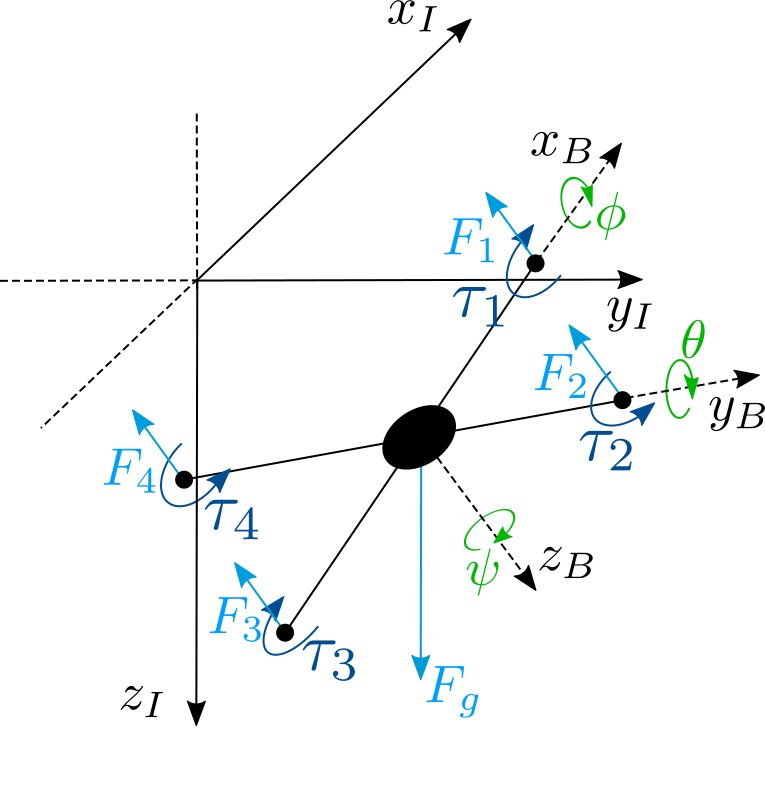
\includegraphics[width=.4\textwidth]{figures/droneDiagram}
	\caption{Forces ($\vec{F}_i$) and torques ($\vec{\tau}_i$) acting on the quadcopter and the positive references chosen for rotations and translations in both inertial and body coordinate frames.}
	\label{droneDiagram}
\end{figure}
%
As it is seen, the system is modeled by using two coordinate frames. The inertial frame is utilized to describe the translational movement while the body frame is attached to the quadcopter and used to characterize its attitude behavior. In the figure, also the positive references for rotational and translational movements are depicted, as well as the main forces and torques acting on the quadcopter. The positive rotations follow a right-hand fashion.

The forces generated in the propeller are readily obtained in the body coordinate frame. In order to represent them in the inertial frame a rotation matrix is used. It is built considering a 123 rotation sequence \cite{rotationmatrix}. This means that any rotation is described as three rotations around the $x_\mathrm{B}$ axis first, then around the $y_\mathrm{B}$ axis and lastly around the $z_\mathrm{B}$ axis. 
 
The dynamic model of the quadcopter is given by three sets of equations. The first describes the motor and the propeller, the second presents the attitude response of the quadcopter and the third explains how the translational variables of the system evolve.

\fxnote{In the modeling section, what are your assumptions? What is the reason for not including model parts such as Gyroscopic torque, Air friction/drag on the quadcopter itself (even though you include it on the propellers), Aerodynamic lift, Mass placement and separation of masses, Coriolis acceleration?}

\subsection{Motor and Propeller}
The four motors in the quadcopter generate a rotation in the propellers that creates the force that lifts the quadcopter. The thrust force can be modeled as proportional to the square of the motor rotational speed. The thrust coefficient for each motor is found experimentally. The units for this coefficient are \si{N s^2 rad^{-2}}
 
The rotation also generates a torque on each motor due to the aerodynamic drag. Drag torque is compensated in the quadcopter by having two of the motors turning in one direction and the two others in the opposite direction. It is as well described as proportional to the square of the rotational speed in terms of a drag coefficient, which is also obtained experimentally. Its units are \si{N m s^2  rad^{-2}}

The expressions for the thrust force and drag torque caused by the rotation of each propeller are
%
\begin{flalign}
	F&=k_{\mathrm{th}}\omega^2\label{eq:thrustForce}\\
	\tau&=k_{\mathrm{d}}\omega^2\label{eq:dragTorque}
\end{flalign}
%
\noindent where $F$ is the thrust force, $k_{th}$ is the thrust coefficient, $\omega$ is the angular speed of the motor, $\tau$ is the drag torque and $k_d$ is the drag coefficient.
%\begin{where}
%  \va{F}{is the thrust force}{N}
%  \va{k_{th}}{is the thrust coefficient}{N\  s^2 \  rad^{-2}}
%  \va{\omega}{is the angular velocity}{rad s^-1}
%  \va{\tau}{is the drag torque}{N m}
%  \va{k_d}{is the drag coefficient}{N \  m\  s^2 \  rad^{-2}}
%\end{where}

These equations are used in the attitude and translational models presented below.
%
\subsection{Attitude Model}
The attitude model equations, which are based on Newton's Second Law for rotational movement, are as follows 
%
\begin{flalign}
	J_x\ddot{\phi}&=k_{\mathrm{th}} (\omega^2_4-\omega^2_2)  L \label{eq:AngleEqVelocities1}\\
	J_y\ddot{\theta}&=k_{\mathrm{th}} (\omega^2_1-\omega^2_3)  L \label{eq:AngleEqVelocities2} \\
	J_z\ddot{\psi}&=k_{\mathrm{d}} (\omega^2_1-\omega^2_2+\omega^2_3-\omega^2_4)\label{eq:AngleEqVelocities3}
\end{flalign}

\noindent where $J_x$, $J_y$ and $J_z$ are the moments of inertia around the three axes of rotation, $\ddot{\phi}$, $\ddot{\theta}$ and $\ddot{\psi}$ are the angular accelerations in roll, pitch and yaw, respectively, $\omega_i$ is the rotational speed of each motor and $L$ is the distance between the center of the quadcopter and the position of the motors.

The expressions above state how the thrust forces and the drag torques generated on the propellers affect the attitude behavior of the quadcopter.  
\subsection{Translational Model}
The equations describing the response of the system along the inertial x, y and z axes are derived from Newton's Second Law of Motion. The forces that act on the system are those from the propellers and the gravitational force. These expressions are
%
\begin{flalign}
     m\ddot{x}_{\mathrm{I}} = &-k_{\mathrm{th}} ({\omega_1}^2+{\omega_2}^2+{\omega_3}^2+{\omega_4}^2) \label{eq:AccelerationEqInertial1}\\
     & \ \times (\cos\phi \sin\theta \cos\psi + \sin\phi\sin\psi)   \nonumber\\
     m \ddot{y}_{\mathrm{I}} = &-k_{\mathrm{th}}({\omega_1}^2+{\omega_2}^2+{\omega_3}^2+{\omega_4}^2) \label{eq:AccelerationEqInertial2}\\
     & \ \times(\cos\phi \sin\theta \sin\psi - \sin\phi \cos\psi)  \nonumber\\
     m\ddot{z}_{\mathrm{I}} = &F_g-k_{\mathrm{th}}\ ({\omega_1}^2+{\omega_2}^2+{\omega_3}^2+{\omega_4}^2) \label{eq:AccelerationEqInertial3}\\
     & \ \times \cos\phi\cos\theta  \nonumber
\end{flalign}
\noindent where $m$ is the mass of the quadcopter, $\ddot{x}_I$, $\ddot{y}_I$ and $\ddot{z}_I$ are the accelerations along the inertial reference frame directions, $\phi$, $\theta$ and $\psi$ are the roll, pitch and yaw angles respectively and $F_g$ is the gravitational force acting on the quadcopter.

It is worth mentioning that, as the thrust forces always point in the negative ${z}_B$ direction, the accelerations along ${x}_{\mathrm{I}}$ and ${y}_{\mathrm{I}}$ directions are zero when pitch and roll angles are zero.

\subsection{Linearization}
The model equations are linearized using the first order Taylor approximation around an equilibrium point of the system. The chosen point is the hovering position, which implies that the attitude and translational accelerations and velocities are zero. The angular position of the quadcopter is also part of the point around which the linearization is made, and it is also set to zero in the three angles.

Choosing a zero acceleration linearization point along the ${z}_{\mathrm{I}}$ axis yields an equilibrium rotational speed so that the necessary thrust is generated to compensate for the gravitational force. The relation is expressed as\fxnote{Should we use the same $\overline{\omega}$?}
\begin{flalign}
    \overline{\omega}_i=\sqrt{\frac{mg}{4k_{th}}}
    \label{eq:equilibriumomegas}
\end{flalign}
The resulting equations for the attitude model after the linearization are 
\begin{flalign}
  J_x \Delta\ddot{\phi}  = &2 k_{\mathrm{th}} L {\overline{\omega}_4} \Delta \omega_4 - 2\ k_{\mathrm{th}} L {\overline{\omega}_2} \Delta \omega_2
  \label{eqAngleLin1} \\
  J_y\Delta\ddot{\theta} =&2 k_{\mathrm{th}} L \overline{\omega}_1 \Delta \omega_1 - 2 k_{\mathrm{th}} L \overline{\omega}_3 \Delta \omega_3
  \label{eqAngleLin2} \\
  J_z\Delta\ddot{\psi}= &2 k_{\mathrm{d}} {\overline{\omega}_1} \Delta \omega_1 - 2 k_{\mathrm{d}}{\overline{\omega}_2} \Delta \omega_2 \label{eqAngleLin3}
  \\ & +\ 2\ k_{\mathrm{d}} {\overline{\omega}_3} \Delta \omega_3 - 2\ k_{\mathrm{d}} {\overline{\omega}_4} \Delta \omega_4\nonumber  
\end{flalign}
\noindent where $\Delta\ddot{\phi}$, $\Delta\ddot{\theta}$ and $\Delta\ddot{\psi}$ are the changes in rotational acceleration from the linearization point, $\overline{\omega}_i$ is the rotational speed of each motor to achieve equilibrium along the $z_\mathrm{I}$ axis and $\Delta \omega_i$ is the change in rotational speed of each motor from the linearization point. 

Similarly, the equations of the translational model are linearized. The result is
\begin{flalign}
  m\Delta\ddot{x}_{\mathrm{I}} =&-k_{\mathrm{th}} ({\overline{\omega}_1}^2+{\overline{\omega}_2}^2+{\overline{\omega}_3}^2+{\overline{\omega}_4}^2) \Delta\theta \label{eq:TransLinearEquations1} \\
  m\Delta\ddot{y}_{\mathrm{I}} = &\ \  \  k_{\mathrm{th}} ({\overline{\omega}_1}^2+{\overline{\omega}_2}^2+{\overline{\omega}_3}^2+{\overline{\omega}_4}^2) \Delta\phi \label{eq:TransLinearEquations2}\\
  m\Delta\ddot{z}_{\mathrm{I}} = &-2 k_{\mathrm{th}}\overline{\omega}_1 \Delta\omega_1 -2 k_{\mathrm{th}} \overline{\omega}_2 \Delta\omega_2 \label{eq:TransLinearEquations3} \\
 &\ \   -2 k_{\mathrm{th}} \overline{\omega}_3 \Delta\omega_3-2 k_{\mathrm{th}} \overline{\omega}_4 \Delta\omega_4 \nonumber 
\end{flalign} 
\noindent where $\Delta\ddot{x_{\mathrm{I}}}$, $\Delta\ddot{y_{\mathrm{I}}}$ and $\Delta\ddot{z_{\mathrm{I}}}$ are the changes in linear acceleration from the linearization point in each direction of the inertial frame and $\Delta \phi$ and $\Delta \theta$ are the changes in roll and pitch from the linearization point, respectively.                %<--subsection
\section{Control}\label{sec:control}\fxnote{Say that we use the network for the design}
The control of the system is divided into two control systems. One handles the attitude and the other controls the translational behavior of the quadcopter. These two are related such that the translational controller sets the references for the angles handled by the inner controller.              %<--subsection
\subsection{Attitude Controller}
The attitude controller for the quadcopter has been designed using a state space representation of the system. This helps handling the coupled angular response of the quadcopter. The chosen states for the system are the three angular positions and the three angular velocities. The input vector of the attitude system consists of the four motor rotational speeds and the output vector consists of the three angles, roll, pitch and yaw. Below, the state, input and the output vectors are presented.
%
\begin{flalign}
	\vec{x}(t) = 
	\begin{bmatrix}
		\phi & \theta & \psi & \dot{\phi} &	\dot{\theta} & \dot{\psi} \\
	\end{bmatrix}	\nonumber
	^T
	\label{xVector}
\end{flalign}  
\begin{flalign}
	\vec{y}(t) = 
	\begin{bmatrix}
		\phi &	\theta & \psi \\
	\end{bmatrix}	\nonumber
	^T
	\label{yVector}
\end{flalign}
\begin{flalign}
	\vec{u}(t)= 
	\begin{bmatrix}
		\omega_1 & \omega_2 &	\omega_3 &	\omega_4 \\
	\end{bmatrix}\nonumber	
	^T
	\label{uVector}+
\end{flalign}
%
The above is then used in construction of the state space matrix representation as displayed in \autoref{xDotSS} and \ref{ySS}.
\begin{flalign}
	\vec{\dot{x}}(t)&=\vec{A} \cdot \vec{x}(t) + \vec{B} \cdot \vec{u}(t)
	\label{xDotSS} 
\end{flalign}
\begin{flalign}
	\vec{y}(t)&=\vec{C} \cdot \vec{x}(t) + \vec{D} \cdot \vec{u}(t)\label{ySS} 
\end{flalign}

Where $\vec{A}$ is the system matrix, $\vec{B}$ is the input matrix, $\vec{C}$ is the output matrix and $\vec{D}$ is the feedback matrix.

The values for the $\vec{A}$, $\vec{B}$, $\vec{C}$ and $\vec{D}$ matrices are obtained from the linearized attitude equations, yielding the matrices shown below. As $\vec{D}$ is a zero matrix, only $\vec{A}$, $\vec{B}$ and $\vec{C}$ are shown. 
\footnotesize
\begin{flalign}   \label{Amatrix}
	\vec{A}=
	\begin{bmatrix}
		\ 0 & 0 & 0 & 1 & 0 & 0     \ \ \ \\ 
		\ 0 & 0 & 0 & 0 & 1 & 0     \ \ \ \\ 
		\ 0 & 0 & 0 & 0 & 0 & 1     \ \ \ \\
		\ 0 & 0 & 0 & 0 & 0 & 0     \ \ \ \\ 
		\ 0 & 0 & 0 & 0 & 0 & 0     \ \ \ \\ 
		\ 0 & 0 & 0 & 0 & 0 & 0     \ \ \  		
	\end{bmatrix}\nonumber
\end{flalign} \label{Bmatrix}
\begin{flalign}
    \vec{B} =
	\begin{bmatrix}
		\ 0 & 0 & 0 & 0      \ \ \ \\ 
		\ 0 & 0 & 0 & 0      \ \ \ \\ 
		\ 0 & 0 & 0 & 0      \ \ \ \\
		\ 0 & \si{-\frac{2 \cdot k_{th} \cdot L \cdot \overline{\omega}_2}{J_x}} & 0 & \si{\frac{2 \cdot k_{th} \cdot L \cdot \overline{\omega}_4}{J_x}}      \ \ \ \\ 
		\ \si{\frac{2 \cdot k_{th} \cdot L \cdot \overline{\omega}_1}{J_y}} & 0 & \si{-\frac{2 \cdot k_{th} \cdot L \cdot \overline{\omega}_3}{J_y}} & 0      \ \ \ \\ 
		\ \frac{2 \cdot k_d \cdot {\overline{\omega}_1}}{J_z} & - \frac{2 \cdot k_d \cdot {\overline{\omega}_2}}{J_z} & \frac{2 \cdot k_d \cdot {\overline{\omega}_3}}{J_z} & - \frac{2 \cdot k_d \cdot {\overline{\omega}_4}}{J_z}      \ \ \ 		
	\end{bmatrix}\nonumber
\end{flalign}
\begin{flalign} \label{Cmatrix}
	\vec{C} =	 
	\begin{bmatrix}
		\ 1 & 0 & 0 & 0 & 0 & 0     \ \ \ \\ 
		\ 0 & 1 & 0 & 0 & 0 & 0     \ \ \ \\ 
		\ 0 & 0 & 1 & 0 & 0 & 0     \ \ \ 		
	\end{bmatrix}\nonumber
\end{flalign}
\normalsize

This system can also be proven to be both controllable and observable, which are necessary conditions to be able to design a observer-based control.

For the quadcopter to hover, it is desired to keep the attitude in equilibrium; this is achieved using a state feedback. To be able to change and track a reference an integral controller is designed combined with the other one. It is also desirable to use an observer in order to estimate the angular velocities that are part of the state of the system. This is done using a reduced-order observer. These two designs can be done independently due to the separation principle. \cite{ssReference}

\autoref{AttitudeControlDiagram} shows how this designs are related.

\begin{figure}[H]
    \centering
    
\includegraphics[scale=0.3]{figures/AttitudeControlDiagram}
    \caption{ Control structure for the system, including the state feedback, the integral control and the reduced order observer.}
    \label{AttitudeControlDiagram}
\end{figure}

%--------------------- StateFeedback with Integral Control ----------------------------
The control design is shown in \autoref{fig:DetailedControllerColorDiagram}.
\begin{figure}[H]
    
\includegraphics[scale=.35]{figures/DetailedControllerColorDiagram}
    \centering
    \captionof{figure}{Detail of the left diagram, that includes all the variables used in the design of the controller.}
    \label{fig:DetailedControllerColorDiagram}
\end{figure}

It can be seen that there are three new states that are added to the system, $\vec{x}_{Int}(t)$ and lead to the extended system shown in \autoref{xdotSSExtended} and \ref{ySSExtended}.
%
\begin{flalign} 
\dot{\vec{x}}_e(t) &= \vec{A}_e \  \vec{x}_e(t) + \vec{B}_e \  \vec{u}(t) + 
\begin{bmatrix}
\ \vec{0}     \ \ \ \\ 
\ \vec{-I}     \ \ \  		
\end{bmatrix}
\vec{r}(t) 
\label{xdotSSExtended}\\ 
\vec{y}(t) &= \vec{C}_e \  \vec{x}_e 
\label{ySSExtended}
\end{flalign} 
%
being\\
\scriptsize
\begin{minipage}{0.28\linewidth}
    \begin{flalign}
    \dot{\vec{x}}_e(t)= 
    \begin{bmatrix}
    \ \dot{\vec{x}}(t)      \ \  \\ 
    \ \dot{\vec{x}}_{Int}(t)      \ \   		
    \end{bmatrix} \nonumber
    \end{flalign}
\end{minipage}\hfill
\begin{minipage}{0.2\linewidth}
    \begin{flalign}
    \vec{A}_e=
    \begin{bmatrix}
    \ \vec{A}  & \vec{0}    \ \  \\ 
    \ \vec{C}  & \vec{0}    \ \   		
    \end{bmatrix} \nonumber
    \end{flalign}
\end{minipage}   \hfill 
\begin{minipage}{0.2\linewidth}
    \begin{flalign}
    \vec{B}_e=
    \begin{bmatrix}
    \ \vec{B}    \ \  \\ 
    \ \vec{0}     \ \   		
    \end{bmatrix} \nonumber
    \end{flalign}
\end{minipage}\hfill
\begin{minipage}{0.2\linewidth}
    \begin{flalign}
    \vec{C}_e=
    \begin{bmatrix}
    \ \vec{C}  & \vec{0}  \ \   		
    \end{bmatrix} \nonumber
    \end{flalign}
\end{minipage}
\normalsize
\\

With this approach, the control law given by \autoref{eq:ssControllerAction}.
%
\begin{flalign} 
    \vec{u}(t) &=\vec{F} \  \vec{x}(t) + \ \vec{F}_{Int} \  \vec{x}_{Int}(t)
    \label{eq:ssControllerAction}
\end{flalign}
%
The resulting feedback law can be design as a conventional state feedback, where the goal is to choose an appropriate $F_e=[F \ F_{Int}]$ matrix such that the eigenvalues of $A_e+B_eF_e$ are the new poles that the system needs to have in order to achieve the desired dynamics.

Once $F_e$ is obtained, it can be split into $F$ and $F_{Int}$ by taking the first 6 columns for the state feedback and the last 3 for the integral control. In this way, the controller can be implemented as shown in \autoref{fig:DetailedControllerColorDiagram}.

%--------------------- Reduced-Order Observer ----------------------------


In general an observer is utilized in a control system if either one of two specific cases occurs. If certain states in the system are not measured, an observer can estimate the unmeasured states by means of the system output and input. However, it is also possible to use an observer if the measured data gathered from the sensors is affected by noise. The observer can thereby use both the noisy measured states and the estimated states creating a filtered version. This case will however not be utilized in the prototype.

With this approach, the first three states, $x_1$ with be equal to the outputs, $y$, whereas the other three states will be estimated, $\hat{x}_2$.

The matrices that define the original system can be split into submatrices, that will be used in the design of the observer, as follows:\\
%
\begin{minipage}{0.45\linewidth}
    \begin{flalign}
    \vec{A}=
    \begin{bmatrix}
    \ \vec{A11}_{3 \times 3}  & \vec{A12}_{3 \times 3}    \ \ \ \\ 
    \ \vec{A21}_{3 \times 3}  & \vec{A22}_{3 \times 3}    \ \ \  		
    \end{bmatrix} \nonumber
    \end{flalign}
\end{minipage}   \hfill 
\begin{minipage}{0.45\linewidth}
    \begin{flalign}
    \vec{B}=
    \begin{bmatrix}
    \ \vec{B1}_{3 \times 4}    \ \ \ \\ 
    \ \vec{B2}_{3 \times 4}     \ \ \  		
    \end{bmatrix} \nonumber
    \end{flalign}
\end{minipage}\hfill
\\

As described in ?? the system is observable, making it possible to find an observer gain, $L_{obs}$, which makes \autoref{eq:observerStable} stable \cite{ssReference}.
%
\begin{flalign}
    \vec{A_{22}} + \vec{L_{obs}}\vec{A_{A12}} \label{eq:observerStable}
\end{flalign}

With this observer gain, the observer in \autoref{eq:observerStable} ensures an estimate $\hat{x}_2$ which converges to $x_2$ at a rate given by the eigenvalues of \autoref{eq:eqobservertheorem}.
\small
\begin{flalign}
    \vec{\hat{\dot{x}}_2} &= \vec{A_{21}}\vec{y} + \vec{A_{22}}\vec{\hat{x}_2} + \vec{B_2u} + \vec{L_{obs}}\vec{(A_{12}\hat{x}_2} - \vec{A_{21}x_2}) \label{eq:eqobservertheorem}
\end{flalign}
\normalsize \\
This estimation of $\hat{x}_2$ can also be seen\autoref{fig:observerDiagram}.
\begin{figure}[H]
    
\includegraphics[scale=.2]{figures/observerDiagram}
    \centering
    \captionsetup{justification=centering}
    \captionof{figure}{This diagram should be made so it looks a bit more similar to the previous on. But only the part with the observer.}
    \label{fig:observerDiagram}
\end{figure}











      %<--subsubsection
\section{Translational Controller} \label{sec:TranslationalController}

General blockdiagram with the controllers and explanation (not in high depth)

\subsection{Controllers for x and y axes}
In this section the governing model equations for the x and y axes is Laplace transformed and put on transfer function. 

For the sake of repetition, the model expression for roll and pitch are as follows:
\begin{align}
m\Delta\ddot{x}_I&= -k_{th}({\overline{\omega}_1}^2+{\overline{\omega}_2}^2+{\overline{\omega}_3}^2+{\overline{\omega}_4}^2)\cos(\overline{\theta})\Delta\theta\\ \label{eq:model_x_transl}
m\Delta\ddot{y}_I&= k_{th}({\overline{\omega}_1}^2+{\overline{\omega}_2}^2+{\overline{\omega}_3}^2+{\overline{\omega}_4}^2)\cos(\overline{\phi})\cos(\overline{\theta})\Delta\phi \label{eq:model_y_transl}
\end{align} 
Laplace transforming \autoref{eq:model_x_transl} and \ref{eq:model_y_transl_y} yield:
\begin{align}
m x_1(s)s^2&=-k_{th}\cdot (\omega_1 ^2 + \omega_2 ^2 + \omega_3 ^2 + \omega_4 ^2) \theta\\
m y_1(s) s^2&= k_{th} (\omega_1 ^2 + \omega_2 ^2 + \omega_3 ^2 + \omega_4 ^2)\phi
\end{align}
It is desirable to have a transfer function where the input is the angle, as this is the output from the attitude controller that goes into the translational controller block. The output of the translational controller must be the velocity in the x and y axes respectively. \\
The transfer functions can now be written as:
\begin{align}
H_{x1}(s)&=\frac{x_1(s) s}{\theta}=\frac{-k_{th} (\omega_1 ^2 + \omega_2 ^2 + \omega_3 ^2 + \omega_4 ^2)}{m s}\label{eq:conHx}\\
H_{y1}(s)&=\frac{y_1(s) s}{\phi}=\frac{k_{th}(\omega_1 ^2 + \omega_2 ^2 + \omega_3 ^2 + \omega_4 ^2)}{m\cdot s}\label{eq:conHy}
\end{align}
\begin{where}
\va{H_{x1}}{is the plant for the translational roll}{1}
\va{H_{y1}}{is the plant for the translational pitch}{1}
\end{where}

From \autoref{eq:conHx} and \ref{eq:conHy} it is clearly seen that the two plants are similar but with different sign of the thrust coefficient. The controller design will be carried out for the translational roll model and applied for the translational pitch model  afterwards.

The systems are first order systems, that has one pole in zero and no zeroes. This means the systems are marginally stable. The roll model expression,\autoref{eq:conHx}, is negative, which requires a negative controller gain to become positive. If this is not done, the controller gain will move the pole to the right half plane, making the system unstable. This is not the case for the pitch model expression, \autoref{eq:conHy}.  

Moreover the zero-pole makes them type 1 systems, which means no steady state error will be present in a step response. 
A proportional controller is considered sufficient, as it does not have to compensate for a steady state error. By increasing the absolute gain value the system will become faster, which is desirable. To determine how large the absolute gain can be without making the system unstable due to saturation issues, it is necessary to consider the bandwidth. \\ \\
The data from the Vicon room is transmitted with 100 Hz. This means the attitude controller must run with 50 Hz as maximum to ensure the controller is slower than the sensor data. A rule of thumb states that the bandwidth of the system shall be 25 times smaller than the attitude controller. The desired bandwidth of the translational roll controller is calculated as follows:
\begin{align}
BW=2\cdot \pi\cdot \frac{f_s}{25}=2\cdot \pi \frac{50}{25}=12.57\label{eq:bw_X}
\end{align}
\begin{where}
\va{BW}{is the bandwidth of the plant}{rad \cdot s^{-1}}
\va{f_s}{is the sampling frequency of the plant}{Hz}
\end{where}

From \autoref{eq:bw_X} it is known, that the ideal bandwidth of the system is 12.57 rad/s. 
\begin{figure}[H]
	\centering
	\includegraphics[width=0.7\textwidth]{figures/bode_x.png}
	\caption{Bodeplot of the plant, with the bandwidth of 12.6 rad/s displayed.}\label{fig:bode_x}
\end{figure}
The bodeplot in \autoref{fig:bode_x} reveals that the magnitude is -2.15 dB at 12.6 rad/s and must be lowered by 0.85 dB. 

The gain of the P-controller is found to be: 
\begin{align}
C_{x,y}=10^{\frac{-0.85}{20}}=0.907\\
\end{align}

The step response for the designed controller can be seen in \autoref{fig:step_x}
\begin{figure}[H]
	\centering
	\includegraphics[width=0.8\textwidth]{figures/step_x.png}
	\caption{Step response for P-controller with a gain of -0.907 and 0.907 for x and y respectively.}\label{fig:step_x}
\end{figure}
When examining \autoref{fig:step_x}it is seen that, as expected,there is no steady state error. The system settles at 0.41 seconds and has a rise time of 0.12 seconds. Both settling time and rise time is within the requirements. As it is a first order system, there is no overshoot and it can therefore be concluded that the P-controller meets all requirements.
\\
\\
Before it can be implemented and tested on the quadcopter, it needs to be discretized. As it is P-controllers, it simply means to encounter the sampling rate. The discretized controllers are presented along with the continuous controller in \fxnote{make graph}.
\\ \\
  
%\subsubsection*{Pitch translational controller}
%The roll and pitch translational models are very similar and will therefore be designed similarly. The design procedure will be the same as for the translational roll controller.\\

% 
%The desired bandwidth is 12,57 rad/s as derived in \autoref{eq:bw_X}. 
%\begin{figure}[H]
%	\centering
%	\includegraphics[width=0.7\textwidth]{figures/bode_y.png}
%	\caption{Bode plot of the plant with the 12.6 bandwidth displayed.}\label{fig:bode_y}
%\end{figure}
%The bode plot in \autoref{fig:bode_z} reveals that the magnitude is -8.2 dB at a magnitude of 12.6 rad/s. The magnitude has to be lifted by 5,2 dB to obtain the desired bandwidth. 




%Before designing the controller limit checks of the transfer function to verify if the model behaves as the plant is expected to in reality is carried out. \\
%\fxfatal{I am having trouble thinking about it, as it is not entirely intuitive to me, when the input is an angle and not a force - however if possible, i think we should have a short piece of text to show we have been critical to the math we have derived - to check it before continuing.} 
%
%Now that the limit checks confirms the sanity of the model, the controller can be designed. \fxnote{I still think that all of the above in this section shall be moved to the model chapter as conclusion of the chapter.}\\
%

%
%FOR NIELS : 
%
%\begin{figure}[H]
%	\centering
%	\includegraphics[width=0.7\textwidth]{figures/bode_z.png}
%	\caption{Bode plot of the plant with the 12.6 bandwidth displayed.}\label{fig:bode_z}
%\end{figure}
%The bode plot in \autoref{fig:bode_z} reveals that the magnitude is -8.2 dB at a magnitude of 12.6 rad/s. The magnitude has to be lifted by 5,2 dB to obtain the desired bandwidth. 
%
%The gain of the P-controller is found to be:
%\begin{align}
%C_y=10^{\frac{5.2}{20}}=1.82
%\end{align}
%The step response can be seen in

%
%The model expression for pitch is previously derived to be:
%\begin{align}
%m\Delta\ddot{y}_I = k_{th}({\overline{\omega}_1}^2+{\overline{\omega}_2}^2+{\overline{\omega}_3}^2+{\overline{\omega}_4}^2)\cos(\overline{\phi})\cos(\overline{\theta})\Delta\phi
%\label{eq:model_y_transl}
%\end{align}
%Laplace transforming \autoref{eq:model_y_transl_y} yields:
%\begin{align}
%m\cdot y_1(s)\cdot s^2= k_{th}\cdot (\omega_1 ^2 + \omega_2 ^2 + \omega_3 ^2 + \omega_4 ^2)\cdot \phi
%\end{align}
%The transfer function for the pitch is as follows:
%\begin{align}
%H_{y1}(s)=\frac{y_1(s)\cdot s}{\phi}=\frac{k_{th}\cdot (\omega_1 ^2 + \omega_2 ^2 + \omega_3 ^2 + \omega_4 ^2)}{m\cdot s}
%\end{align}
%\begin{where}
%\va{H_{y1}}{is the plant for the translational pitch}{1}
%\end{where}


\subsection{Controller for z axis}
Derivation of the transfer function 



Root locus and bode

Problem with P controller (Input disturbance)

Simulation of P controller

New controller 

simulation of New controller

 %<--subsubsection
%
%-----RESULTS-----------------------------------------------------------
\section{Results}

The controllers have been simulated in MATLAB Simulink in order to generate results presented in this section. 

The model parameters can be seen in \autoref{ParametersQuadcopter}. All of them have been obtained through test but the moments of inertia, which were calculated with following an analytical procedure.

\begin{table}[H]
    \centering
    \begin{tabular}{c|c|c}
        %------------------------------------------------------------------------------------------
        \textbf{Symbol} &\textbf{Value} &\textbf{Units}\\
        \hline %-----------------------------------------------------------------------------------
        $m$ & 0.996       &$kg$\\
        \hline %-----------------------------------------------------------------------------------
        $L$  &   0.225       & $m$\\
        \hline %-----------------------------------------------------------------------------------
        $J_x$  & 0.01073       & $kg \  m^2$\\
        \hline %-----------------------------------------------------------------------------------
        $J_y$  & 0.01073       & $kg \  m^2$\\
        \hline %-----------------------------------------------------------------------------------
        $J_z$  & 0.02135       & $kg \  m^2$\\
        \hline %-----------------------------------------------------------------------------------
        $k_{th}$  & 1.32922\ $10^{-5}$       & $N \  s^2 \  rad^{-2}$\\
        \hline %-----------------------------------------------------------------------------------
        $k_{d}$  & 9.39741\ $10^{-7}$       & $N \  m \  s^2 \  rad^{-2}$\\
        \hline %-----------------------------------------------------------------------------------
        $\overline{\omega}_i$& 429      & $rad \ s^{-1}$\\
        
    \end{tabular}
    \caption{Parameters used though the analysis and design.}

    \label{ParametersQuadcopter}
\end{table}
The attitude controller is defined chosen feedback and integral poles and the observer poles. These are chosen to be $[-6 -6.2 -6.4 -6.6 -6.8 -7 -7.2 -7.4 -7.6]$ and $[-20 -25 30]$ respectively.

The translation velocity controllers of the x and y translational are $C_{\dot{x}}(s)= -0.1$, $C_{\dot{y}}(s)= 0.1$ and the position ones are $C_x(s)= 0.5$, $C_y(s)= 0.5$. The inner loop proportional controller of the z translational cascade controller is
$C_{\dot{z}}(s)=\frac{-201s+0.8}{s}$ and the outer loop is $C_z=0.9$

This controllers have been discretized using th Tustin method with a sampling period of 30 ms. 

Regarding the network, the mean delay selected is 30 ms and the package loss probability has been set to 0 due to the low sending frequency used in the system.
The simulation results obtained with these parameters and controllers are shown in \autoref{PositionControl}.
\begin{figure}[H]
	\centering
	\includegraphics[scale=0.55]{figures/PositionControl}
	\caption{Position control results in the three inertial axes directions. The references given to the control system are shown with dashed lines.}
	\label{PositionControl}
\end{figure}

The inner attitude controller results are also included and shown in \autoref{AttitudeControl}, so the performance of the attitude control can be evaluated. 
\begin{figure}[H]
	\centering
	\includegraphics[scale=0.55]{figures/AttitudeControl}
	\caption{Attitude control results in the three angles. The references given to the attitude control system are shown with dashed lines.}
	\label{AttitudeControl}
\end{figure}



%
%-----DISCUSSION--------------------------------------------------------
\section{Discussion}\label{sec:discussion}

The results obtained show both the attitude and simulated position response of the quadcopter. 

It is seen that the controllers track the references even though the network delay and the sampling rate affects their performance. The network limits the designed bandwidths, especially for the attitude controller. This is due to the limited frequency in which the sensor data is obtained from the motion tracking system. A faster response is achievable if on board sensors for acquiring the attitude are utilized.

Experimental results could not be presented for the translational controllers, as it has not been possible to implement them with success in due time. The design is however deemed reasonable, as simulations show that the design should work in reality. The attitude controller is implemented and achieves the given references.

%Experimental results could not be presented for the translational controllers. As the attitude design has been validated with the same simulation and it works in reality, it can be suggested that it is not the design but the implementation of the translational controllers which, at this point in the design process prevents the realization of a flying quadcopter.
%
%Simple model
%Translational 
%The attitude controller tracks the given references in roll and pitch. The network delay 
%It is also worth observing how the attitude controller shows a permanent error with respect to the reference. This is generated as a result of the integral controller design because it assumes a constant reference applied to it. This issue, though, does not affect the final position of the quadcopter.
%\fxnote{why the controllers are slow?, the delay is high}
%
%-----CONCLUSION--------------------------------------------------------
\section{Conclusion}
The behavior of a quadcopter has been modeled by first principles of physics. A control system has been designed in order to hover and move to a desired position.
The control system has been split into an attitude and a translational controller. The first one has been designed using a state space approach, including state feedback with integral control and a reduced order observer. The translational control system has been designed with a classical control approach and result in three cascade loops, including proportional and PI controllers. 
As the quadcopter uses an external motion tracking system to determine its position and orientation, an analysis of the issues that can arise when having a networked distributed system has been done in order to ensure the control system remains stable. The results obtained from the design show that both the attitude and the translational behavior of the quadcopter has been successfully controlled.


%---------------------------------------------------------
%
%FUTURE WORK---------------------------------------------
\section{Future Work}
Several actions can be done in order to optimize this prototype. The most significant is to implement on board sensors such that the quadcopter will not be limited to only operate within the Vicon room. Hereafter there is a wide range of potential applications that can be enforced.


%
%-----ACKNOWLEDGMENTS---------------------------------------------------
%\section{Acknowledgments}\label{sec:acknowledgements}
%Henrik Schiøler , associated professor at Aalborg University \\
%Christoffer Sloth, associated professor at Aalborg University
%\fxnote{Acknowledgements}
%
%-----BIBLIOGRAPHY------------------------------------------------------
\printbibliography

\end{document}